% ==========================================
% CHAPITRE 5 — ÉTUDE DU SPRINT 3
% Corrigé selon rapport de jury
% ==========================================
\newpage
\chapter{ÉTUDE DU SPRINT 3}

\noindent \textbf{\Large Plan}
\vspace{0.8cm}

\begin{enumerate}[label=\textbf{\arabic*}, leftmargin=1.5cm, labelsep=0.8cm]
    \item[] \hspace*{-1.5cm}\textbf{Introduction}                        \dotfill \pageref{sec:s3-intro}
    \item \textbf{User Stories du troisième sprint}                       \dotfill \pageref{sec:s3-userstories}
    \item \textbf{Backlog du troisième Sprint}                            \dotfill \pageref{sec:s3-backlog}
    \item \textbf{Spécification fonctionnelle}                            \dotfill \pageref{sec:s3-specification}
    \item \textbf{Conception du Sprint 3}                                 \dotfill \pageref{sec:s3-conception}
    \item \textbf{Étude et réalisation}                                   \dotfill \pageref{sec:s3-realisation}
    \item \textbf{Tests et Validation}                                    \dotfill \pageref{sec:s3-tests}
    \item \textbf{Rituels Agiles et Clôture du Sprint}                    \dotfill \pageref{sec:s3-rituels}
    \item[] \hspace*{-1.5cm}\textbf{Conclusion}                          \dotfill \pageref{sec:s3-conclusion}
\end{enumerate}
\vfill
\newpage

% ============================================================
\section*{Introduction}
\label{sec:s3-intro}
\addcontentsline{toc}{section}{Introduction}
% ============================================================

S'appuyant sur le référentiel de données consolidé lors des phases
précédentes, ce chapitre présente les réalisations du Sprint~3, qui
constitue le c\oe{}ur métier différenciant de la plateforme PaieZone~RH.
Cette itération est dédiée à l'automatisation de la paie et à la gestion
du temps, intégrant le paramétrage réglementaire tunisien, le calcul des
bulletins de paie, les déclarations sociales (CNSS) ainsi que le suivi
des congés et des absences.

Le présent chapitre suit la structure agile standard des chapitres
précédents~: spécification via les User Stories et le Sprint Backlog,
modélisation UML (cas d'utilisation, classes, séquences), réalisation
des interfaces Angular, validation par plan de tests multiniveaux,
puis clôture agile (Sprint Review et Rétrospective).

% ============================================================
\section{User Stories du troisième sprint}
\label{sec:s3-userstories}
% ============================================================

Le tableau~\ref{tab:us-sprint3} présente les vingt-deux User Stories
identifiées pour le Sprint~3 de PaieZone, réparties sur trois domaines
fonctionnels~: la gestion des paramètres réglementaires, la gestion
de la paie et la gestion des congés et des absences.

\begin{small}
\renewcommand{\arraystretch}{1.4}
\begin{longtable}{|>{\bfseries}p{1.2cm}|p{9.5cm}|>{\centering\arraybackslash}p{2.5cm}|}
\hline
\rowcolor[gray]{0.9} \textbf{ID} & \textbf{User Story} & \textbf{Priorité} \\ \hline
\endfirsthead
\hline
\rowcolor[gray]{0.9} \textbf{ID} & \textbf{User Story} & \textbf{Priorité} \\ \hline
\endhead
\hline
\endfoot
\hline
\caption{User Stories du Sprint 3 }
\label{tab:us-sprint3}
\endlastfoot

10.1 & En tant que Super Admin, je souhaite \textbf{consulter la liste des paramètres réglementaires} afin de vérifier les taux légaux en vigueur. & Haute \\ \hline
10.2 & En tant que Super Admin, je souhaite \textbf{ajouter un nouveau paramètre réglementaire} afin d'intégrer une nouvelle règle légale dans le système. & Haute \\ \hline
10.3 & En tant que Super Admin, je souhaite \textbf{modifier un paramètre réglementaire} afin de mettre à jour les taux conformément aux évolutions législatives. & Haute \\ \hline
10.4 & En tant que Super Admin, je souhaite \textbf{consulter l'historique des modifications des paramètres} afin de garantir la traçabilité des changements réglementaires. & Moyenne \\ \hline
11.1 & En tant que RH, je souhaite \textbf{créer une période de paie} afin de lancer le cycle de traitement des salaires. & Critique \\ \hline
11.2 & En tant que RH, je souhaite \textbf{modifier une période de paie} afin de corriger les données avant la clôture. & Haute \\ \hline
11.3 & En tant que RH, je souhaite \textbf{clôturer une période de paie} afin de valider les calculs et de bloquer toute modification ultérieure. & Critique \\ \hline
11.4 & En tant que RH, je souhaite \textbf{lancer le calcul de tous les bulletins d'une période} afin de générer automatiquement les salaires nets de l'ensemble du personnel. & Critique \\ \hline
11.5 & En tant que RH, je souhaite \textbf{créer une rubrique de paie} afin de structurer les éléments de calcul du salaire. & Haute \\ \hline
11.6 & En tant que RH, je souhaite \textbf{modifier une rubrique de paie} afin de l'adapter aux besoins de la société. & Moyenne \\ \hline
11.7 & En tant que RH, je souhaite \textbf{ajouter une prime} à un employé afin d'augmenter sa rémunération pour une période donnée. & Haute \\ \hline
11.8 & En tant que RH, je souhaite \textbf{modifier une prime} afin d'ajuster son montant avant le calcul de la paie. & Moyenne \\ \hline
11.9 & En tant que RH, je souhaite \textbf{valider une demande d'avance} afin d'accorder le soutien financier sollicité par l'employé. & Haute \\ \hline
11.10 & En tant que RH, je souhaite \textbf{refuser une demande d'avance} afin d'informer l'employé du rejet de sa demande. & Haute \\ \hline
11.11 & En tant qu'Employé, je souhaite \textbf{demander une avance sur salaire} afin de recevoir un soutien financier ponctuel. & Haute \\ \hline
11.12 & En tant que RH, je souhaite \textbf{générer un bulletin de paie} afin de le distribuer à l'employé concerné. & Critique \\ \hline
11.13 & En tant que RH, je souhaite \textbf{générer un fichier CNSS} afin de déclarer les salariés auprès de la Caisse Nationale de Sécurité Sociale. & Critique \\ \hline
12.1 & En tant que RH, je souhaite \textbf{créer un type de congé} afin de définir les règles et les quotas associés. & Haute \\ \hline
12.2 & En tant qu'Employé, je souhaite \textbf{demander un congé} afin de m'absenter légitimement de mon poste de travail. & Haute \\ \hline
12.3 & En tant que RH, je souhaite \textbf{valider une demande de congé} afin de gérer la disponibilité et la continuité du service. & Haute \\ \hline
12.4 & En tant qu'Employé, je souhaite \textbf{consulter mon solde de congé} afin de planifier mes absences en connaissance de cause. & Haute \\ \hline
12.5 & En tant que RH, je souhaite \textbf{gérer les jours fériés} afin de les intégrer automatiquement dans le calcul de la paie et dans la gestion des congés. & Moyenne \\

\end{longtable}
\end{small}
\renewcommand{\arraystretch}{1.0}

% ============================================================
\section{Backlog du troisième Sprint}
\label{sec:s3-backlog}
% ============================================================

Le Tableau~\ref{tab:backlog-sprint3} détaille le backlog complet du
troisième Sprint, regroupant la gestion des paramètres réglementaires,
le traitement de la paie, ainsi que le suivi des congés et des absences.

\begin{small}
\renewcommand{\arraystretch}{1.4}
\begin{longtable}{|>{\raggedright\arraybackslash}p{2.8cm}|>{\raggedright\arraybackslash}p{6.2cm}|>{\raggedright\arraybackslash}p{6.2cm}|c|}

\hline
\rowcolor[gray]{0.9} \textbf{Item} & \textbf{User Story} & \textbf{Tâches} & \makecell{\textbf{Est.}\\\textbf{(j)}} \\ \hline
\endfirsthead
\hline
\rowcolor[gray]{0.9} \textbf{Item} & \textbf{User Story} & \textbf{Tâches} & \makecell{\textbf{Est.}\\\textbf{(j)}} \\ \hline
\endhead
\hline
\endfoot
\hline
\caption{Backlog détaillé du troisième Sprint}
\label{tab:backlog-sprint3} 
\endlastfoot

\multirow{4}{*}{\makecell[c]{\textbf{Gestion des}\\ \textbf{Paramètres}\\ \textbf{Réglementaires}}}
& \textbf{10.1} En tant que Super Admin, je souhaite consulter la liste des paramètres réglementaires afin de vérifier les taux légaux en vigueur.
& - Concevoir l'interface de consultation des paramètres réglementaires.\newline
- Développer l'API REST de récupération des paramètres actifs.
& \textbf{1} \\ \cline{2-4}

& \textbf{10.2} En tant que Super Admin, je souhaite ajouter un nouveau paramètre réglementaire afin d'intégrer une nouvelle règle légale.
& - Développer le formulaire d'ajout d'un paramètre (taux, date d'entrée en vigueur).\newline
- Implémenter l'API REST d'insertion avec versionnage.\newline
- Tester la prise en compte du nouveau taux dans les calculs de paie.
& \textbf{1} \\ \cline{2-4}

& \textbf{10.3} En tant que Super Admin, je souhaite modifier un paramètre réglementaire afin de mettre à jour les taux conformément aux évolutions législatives.
& - Développer l'interface de modification du paramètre.\newline
- Implémenter la traçabilité des modifications dans le journal d'audit.\newline
- Tester l'impact de la mise à jour sur les calculs historiques.
& \textbf{1} \\ \cline{2-4}

& \textbf{10.4} En tant que Super Admin, je souhaite consulter l'historique des modifications des paramètres afin de garantir la traçabilité des changements réglementaires.
& - Créer l'interface de consultation de l'historique des paramètres.\newline
- Développer l'API REST de récupération des versions antérieures.
& \textbf{1} \\ \hline

\multirow{3}{*}{\makecell[c]{\textbf{Gestion des}\\ \textbf{Périodes}\\ \textbf{de Paie}}}
& \textbf{11.1} En tant que RH, je souhaite créer une période de paie afin de lancer le cycle de traitement des salaires.
& - Concevoir l'interface de création d'une période de paie (mois, année).\newline
- Développer l'API REST de création de la période.\newline
- Tester les contraintes de dates et l'unicité de la période.
& \textbf{1} \\ \cline{2-4}

& \textbf{11.2} En tant que RH, je souhaite modifier une période de paie afin de corriger les données avant la clôture.
& - Développer l'interface de modification de la période.\newline
- Implémenter les contrôles de modification (période non clôturée uniquement).\newline
- Tester les transitions de statut.
& \textbf{1} \\ \cline{2-4}

& \textbf{11.3} En tant que RH, je souhaite clôturer une période de paie afin de valider les calculs et de bloquer toute modification ultérieure.
& - Implémenter le verrouillage de la période et de tous ses bulletins.\newline
- Développer l'API REST de clôture avec horodatage .\newline
- Tester le blocage effectif des modifications post-clôture.
& \textbf{1} \\ \hline

\multirow{1}{*}{\makecell[c]{\textbf{Calcul des}\\ \textbf{Bulletins}\\ \textbf{de Paie}}}
& \textbf{11.4} En tant que RH, je souhaite lancer le calcul de tous les bulletins d'une période afin de générer automatiquement les salaires nets de l'ensemble du personnel.
& - Implémenter le moteur de calcul du salaire net (rubriques, cotisations CNSS/CAVIS/CSS, IRPP, primes, avances).\newline
- Implémenter le traitement en lot.\newline

- Intégrer les paramètres réglementaires dans le moteur de calcul.\newline
- Tester les cas limites (prime, avance, mi-temps).
& \textbf{5} \\ \hline

\multirow{4}{*}{\makecell[c]{\textbf{Rubriques}\\ \textbf{\& Primes}}}
& \textbf{11.5} En tant que RH, je souhaite créer une rubrique de paie afin de structurer les éléments de calcul du salaire.
& - Concevoir l'interface de création d'une rubrique (type, montant, nature : gain/retenue).\newline
- Développer l'API REST d'insertion de la rubrique.\newline
- Tester la prise en compte de la rubrique dans le calcul du bulletin.
& \textbf{1} \\ \cline{2-4}

& \textbf{11.6} En tant que RH, je souhaite modifier une rubrique de paie afin de l'adapter aux besoins de la société.
& - Développer l'interface de modification de la rubrique.\newline
- Implémenter la mise à jour en base avec contrôle de cohérence.
& \textbf{1} \\ \cline{2-4}

& \textbf{11.7} En tant que RH, je souhaite ajouter une prime à un employé afin d'augmenter sa rémunération pour une période donnée.
& - Développer l'interface et l'API REST de création d'une prime individuelle.\newline
- Tester l'intégration de la prime dans le calcul du bulletin.
& \textbf{1} \\ \cline{2-4}

& \textbf{11.8} En tant que RH, je souhaite modifier une prime afin d'ajuster son montant avant le calcul de la paie.
& - Développer l'interface de modification de la prime.\newline
- Implémenter la mise à jour avec contrôle du statut de la période.
& \textbf{1} \\ \hline

\multirow{3}{*}{\makecell[c]{\textbf{Gestion}\\ \textbf{des Avances}}}
& \textbf{11.9} En tant que RH, je souhaite valider une demande d'avance afin d'accorder le soutien financier sollicité par l'employé.
& - Implémenter le workflow de validation par le RH.\newline
- Mettre à jour le statut en "APPROVED".\newline
- Tester la déduction automatique de l'avance dans le bulletin.
& \textbf{1} \\ \cline{2-4}

& \textbf{11.10} En tant que RH, je souhaite refuser une demande d'avance afin d'informer l'employé du rejet.
& - Implémenter le workflow de refus avec saisie obligatoire d'une raison.\newline
- Mettre à jour le statut en "REJECTED".\newline
- Tester la notification de refus à l'employé.
& \textbf{1} \\ \cline{2-4}

& \textbf{11.11} En tant qu'Employé, je souhaite demander une avance sur salaire afin de recevoir un soutien financier ponctuel.
& - Développer l'interface de demande d'avance (formulaire employé : montant, raison).\newline
- Implémenter les contrôles (contrat actif, plafond autorisé).\newline
- Tester le cycle complet de la demande à la déduction.
& \textbf{1} \\ \hline

\multirow{2}{*}{\makecell[c]{\textbf{Génération}\\ \textbf{des Documents}\\ \textbf{de Paie}}}
& \textbf{11.12} En tant que RH, je souhaite générer un bulletin de paie afin de le distribuer à l'employé concerné.
& - Concevoir et implémenter le template PDF du bulletin de paie.\newline
- Développer le service de génération PDF.\newline
- Implémenter la mise à disposition du bulletin dans l'espace employé.\newline
- Tester la conformité du PDF avec les paramètres réglementaires.
& \textbf{2} \\ \cline{2-4}

& \textbf{11.13} En tant que RH, je souhaite générer un fichier CNSS afin de déclarer les salariés auprès de la Caisse Nationale de Sécurité Sociale.
& - Développer le service de génération du fichier CNSS au format réglementaire.\newline
- Agréger les montants CNSS salarié et patronal par employé.\newline
- Tester la conformité du fichier généré avec les exigences légales.
& \textbf{2} \\ \hline

\multirow{5}{*}{\makecell[c]{\textbf{Gestion des}\\ \textbf{Congés \&}\\ \textbf{Absences}}}
& \textbf{12.1} En tant que RH, je souhaite créer un type de congé afin de définir les règles et les quotas associés.
& - Concevoir l'interface de création d'un type de congé (annuel, maladie, sans solde).\newline
- Développer l'API REST d'insertion avec gestion des quotas.
& \textbf{1} \\ \cline{2-4}

& \textbf{12.2} En tant qu'Employé, je souhaite demander un congé afin de m'absenter légitimement de mon poste de travail.
& - Développer l'interface de demande de congé (formulaire, calendrier).\newline
- Implémenter les contrôles de solde et de chevauchement.\newline
- Tester la création de la demande avec le statut \texttt{PENDING}.
& \textbf{1} \\ \cline{2-4}

& \textbf{12.3} En tant que RH, je souhaite valider une demande de congé afin de gérer la disponibilité et la continuité du service.
& - Implémenter le workflow de validation/refus par le RH avec notification.\newline
- Mettre à jour automatiquement le solde après approbation.\newline
- Tester la décrémentation du solde.
& \textbf{1} \\ \cline{2-4}

& \textbf{12.4} En tant qu'Employé, je souhaite consulter mon solde de congé afin de planifier mes absences en connaissance de cause.
& - Développer l'interface de consultation du solde de congé par type.\newline
- Développer l'API REST de récupération du solde en temps réel.
& \textbf{1} \\ \cline{2-4}

& \textbf{12.5} En tant que RH, je souhaite gérer les jours fériés afin de les intégrer automatiquement dans le calcul de la paie et dans la gestion des congés.
& - Implémenter la gestion des jours fériés (ajout, suppression).\newline
- Intégrer l'exclusion automatique des jours fériés dans le décompte des congés.\newline
- Tester la prise en compte des jours fériés dans le calcul de paie.
& \textbf{1} \\ \hline

\end{longtable}
\end{small}
\renewcommand{\arraystretch}{1.0}
\normalsize

% ============================================================
\section{Spécification fonctionnelle}
\label{sec:s3-specification}
% ============================================================

La spécification fonctionnelle du Sprint~3 formalise les besoins
exprimés par le Product Owner autour des trois épopées majeures de
ce sprint. Les exigences déjà recueillies dans les User Stories et
le Backlog sont ici modélisées par les diagrammes UML correspondants
et leurs descriptions textuelles contractuelles.

% -----------------------------------------------------------
\subsection{Diagramme de cas d'utilisation du Sprint 3}
% -----------------------------------------------------------

\begin{figure}[H]
  \centering
  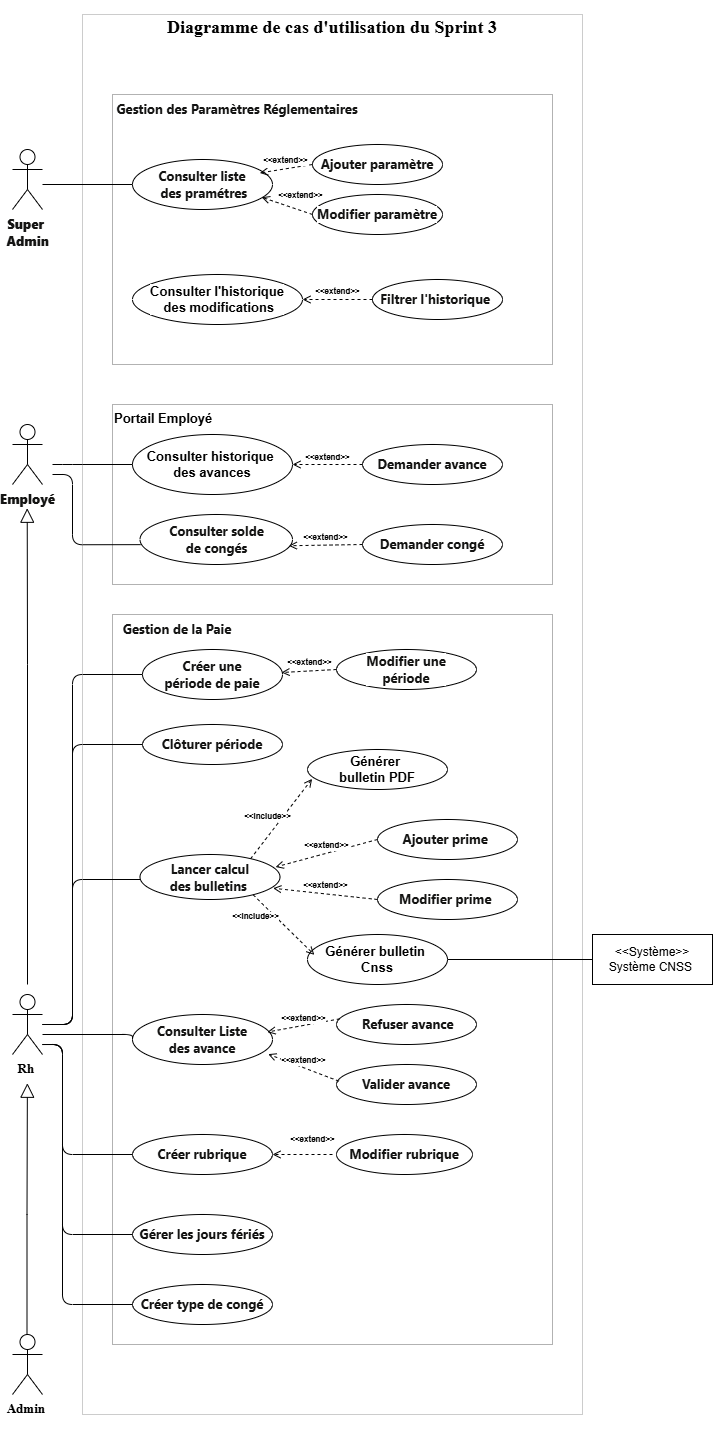
\includegraphics[width=0.69\textwidth]{use-case-sp3.png}
  \caption{Diagramme de cas d'utilisation du Sprint~3}
  \label{fig:uc-sprint3}
\end{figure}

Le diagramme de cas d'utilisation du Sprint~3 organise les fonctionnalités
en trois packages distincts, chacun associé à des acteurs définis~:

\begin{itemize}[label=\textbullet, leftmargin=0.6cm]
    \item \textbf{Gestion des paramètres réglementaires~:}
          Réservé exclusivement au Super Admin, 
          ce module gère les constantes légales configurables 
          sans redéploiement : le taux CNSS salarié, le taux CNSS
           patronal, le taux CAVIS, la CSS, la TFP, le barème IRPP
            progressif (Loi de Finances), et le SMIG. Chaque modification
             est versionnée et tracée dans le journal d’audit.

    \item \textbf{Gestion de la paie~:}
          Le RH Comptable pilote l'intégralité du cycle~:
          création et gestion des périodes de paie, configuration des
          rubriques et des éléments variables (primes, rubriques gain/
          retenue), lancement du calcul en lot, génération des bulletins
          PDF et du fichier de déclaration CNSS.
          L'Employé dispose d'un accès limité pour soumettre
          ses demandes d'avance sur salaire.

    \item \textbf{Gestion des congés et des absences~:}
          Le RH Comptable administre les types de congés
          (annuel, maladie, sans solde) et les jours fériés, et valide
          ou refuse les demandes soumises. L'Employé peut
          soumettre une demande de congé et consulter son solde en temps réel.
\end{itemize}

% -----------------------------------------------------------
\subsection{Description textuelle des cas d'utilisation}
% -----------------------------------------------------------

Les descriptions textuelles suivantes formalisent les scénarios des
cas d'utilisation principaux du Sprint~3. Elles constituent la
référence contractuelle de validation avec le Product Owner lors de
la Sprint Review.
\subsubsection{Cas d'utilisation 1 : Lancer le calcul de tous les bulletins d'une période}

Le tableau~\ref{tab:cu-calcul} présente la description textuelle détaillée
du cas d'utilisation « Lancer le calcul des bulletins de paie ».
\mbox{}\\

\begin{xltabular}{\textwidth}{|l|X|}
\hline
\rowcolor[gray]{0.9} \textbf{Élément} & \textbf{Description} \\ \hline
\endfirsthead
\hline
\caption{Description textuelle du CU~: Lancer le calcul des bulletins de paie}
\label{tab:cu-calcul} 
\endlastfoot
\textbf{Titre} & Lancer le calcul de tous les bulletins d'une période \\ \hline
\textbf{Acteur principal} & RH Comptable \\ \hline
\textbf{Préconditions} & Une période de paie existe au statut OUVERTE
  (non clôturée). Des employés actifs sont rattachés à la société.
  Les paramètres réglementaires (taux CNSS, barème IRPP, CSS) sont
  configurés par le Super Admin. \\ \hline
\textbf{Postconditions} & Tous les bulletins  sont générés
  au statut CALCULÉ. La période de paie passe au statut
 CALCULÉE. \\ \hline
\textbf{Scénario principal} &
    \begin{enumerate}[nosep, leftmargin=*]
        \item Le RH accède au module de paie et sélectionne une période en cours.
        \item Il clique sur « Lancer le calcul ».
        \item Le système vérifie que la période est modifiable.
        \item Le système récupère les données de rémunération, de temps de travail et d'absences de chaque employé.
        \item Le système calcule automatiquement les cotisations, les impôts et le salaire net.
        \item Le système génère et enregistre les bulletins de paie de tous les employés.
        \item Le système met à jour le statut de la période.
        \item Le système affiche un résumé global de l'opération au RH.
    \end{enumerate} 
 \\\hline
\textbf{Scénarios alternatifs}
& \textbf{A1~: Période clôturée}~$\rightarrow$ Le système bloque l'action et informe le RH. \\ \cline{2-2}
& \textbf{A2~: Aucun employé actif}~$\rightarrow$ Avertissement affiché, aucun bulletin créé. \\ \cline{2-2}
& \textbf{A3~: Paramètres réglementaires manquants}~$\rightarrow$ Erreur bloquante invitant le Super Admin à configurer les taux. \\
\end{xltabular}

\subsubsection{Cas d'utilisation 2 : Clôturer une période de paie}
Le tableau~\ref{tab:cu-cloture} présente la description textuelle détaillée
du cas d'utilisation « Clôturer une période de paie ».
\mbox{}\\
\begin{xltabular}{\textwidth}{|l|X|}

\hline
\rowcolor[gray]{0.9} \textbf{Élément} & \textbf{Description} \\ \hline
\endfirsthead
\hline
\caption{Description textuelle du CU~: Clôturer une période de paie}
\label{tab:cu-cloture}
\endlastfoot
\textbf{Titre} & Clôturer une période de paie \\ \hline
\textbf{Acteur principal} & RH \\ \hline
\textbf{Préconditions} & La période est au statut CALCULÉE. Tous les bulletins sont calculés. \\ \hline
\textbf{Postconditions} & La période passe au statut CLÔTURÉE . Aucune modification n'est possible. \\ \hline
\textbf{Scénario principal} &
\begin{enumerate}[nosep, leftmargin=*]
    \item Le RH accède à la liste des périodes de paie et sélectionne une période au statut CALCULÉE.
    \item Il clique sur « Clôturer la période ».
    \item Le système vérifie que tous les bulletins associés sont au statut CALCULÉ.
    \item Il verrouille tous les bulletins (CLÔTURÉ) et la période .
    \item Un message de confirmation s'affiche.
\end{enumerate} \\ \hline
\textbf{Scénarios alternatifs}
& \textbf{A1~: Bulletins non finalisés}~$\rightarrow$ Des bulletins sont encore en statut non calculé, le système bloque l'action avec un message d'erreur. \\ \cline{2-2}
& \textbf{A2~: Période déjà clôturée}~$\rightarrow$ Le système affiche un message informatif. \\
\end{xltabular}

\subsubsection{Cas d'utilisation 3 : Demande et traitement d'une avance sur salaire}

Le tableau~\ref{tab:cu-avance} présente la description textuelle détaillée
du cas d'utilisation « Demande et traitement d'une avance sur salaire ».
\mbox{}\\
\begin{xltabular}{\textwidth}{|l|X|}

\hline
\rowcolor[gray]{0.9} \textbf{Élément} & \textbf{Description} \\ \hline
\endfirsthead
\hline
\caption{Description textuelle du CU~: Demande et traitement d'une avance sur salaire}
\label{tab:cu-avance} 
\endlastfoot
\textbf{Titre} & Demande et traitement d'une avance sur salaire \\ \hline
\textbf{Acteurs principaux} & Employé (demandeur) --- RH Comptable (valideur) \\ \hline
\textbf{Préconditions} & L'employé possède un contrat actif. La période de paie est OUVERTE. Aucune avance en statut PENDING n'est en cours. \\ \hline
\textbf{Postconditions} & L'avance est au statut APPROVED et sera déduite du prochain bulletin, ou au statut REJECTED avec une raison enregistrée. \\ \hline
\textbf{Scénario principal} &
\begin{enumerate}[nosep, leftmargin=*]
    \item L'employé accède au module « Mes demandes d'avance ».
    \item Il renseigne le montant, la raison et la date de demande.
    \item Le système vérifie le contrat actif et le plafond autorisé.
    \item L'avance est créée avec le statut PENDING.
    \item Le RH consulte la liste des demandes en attente.
    \item Il sélectionne une demande et clique sur « Approuver ».
    \item Le système met à jour le statut $\rightarrow$ APPROVED.
    \item L'avance sera marquée DEDUCTED lors du calcul du bulletin.
\end{enumerate} \\ \hline
\textbf{Scénarios alternatifs}
& \textbf{A1~: Refus par le RH}~$\rightarrow$ Le RH saisit une raison et clique sur « Refuser », le système passe le statut à REJECTED. \\ \cline{2-2}
& \textbf{A2~: Montant invalide}~$\rightarrow$ Le montant dépasse le plafond autorisé, le système bloque la validation à la soumission. \\
\end{xltabular}

% ============================================================
\section{Conception du Sprint 3}
\label{sec:s3-conception}
% ============================================================

La phase de conception du Sprint~3 traduit les exigences fonctionnelles
en structures techniques. Elle couvre le diagramme de classes enrichi
des nouvelles entités métier introduites dans ce sprint, ainsi que les
diagrammes de séquence des scénarios principaux.

% -----------------------------------------------------------
\subsection{Diagramme de classes}
\label{sec:s3-classes}
% -----------------------------------------------------------

La figure~\ref{fig:classes-sprint3} présente le diagramme de classes
du Sprint~3 de PaieZone.

\newpage
\begin{figure}[H]
  \centering
  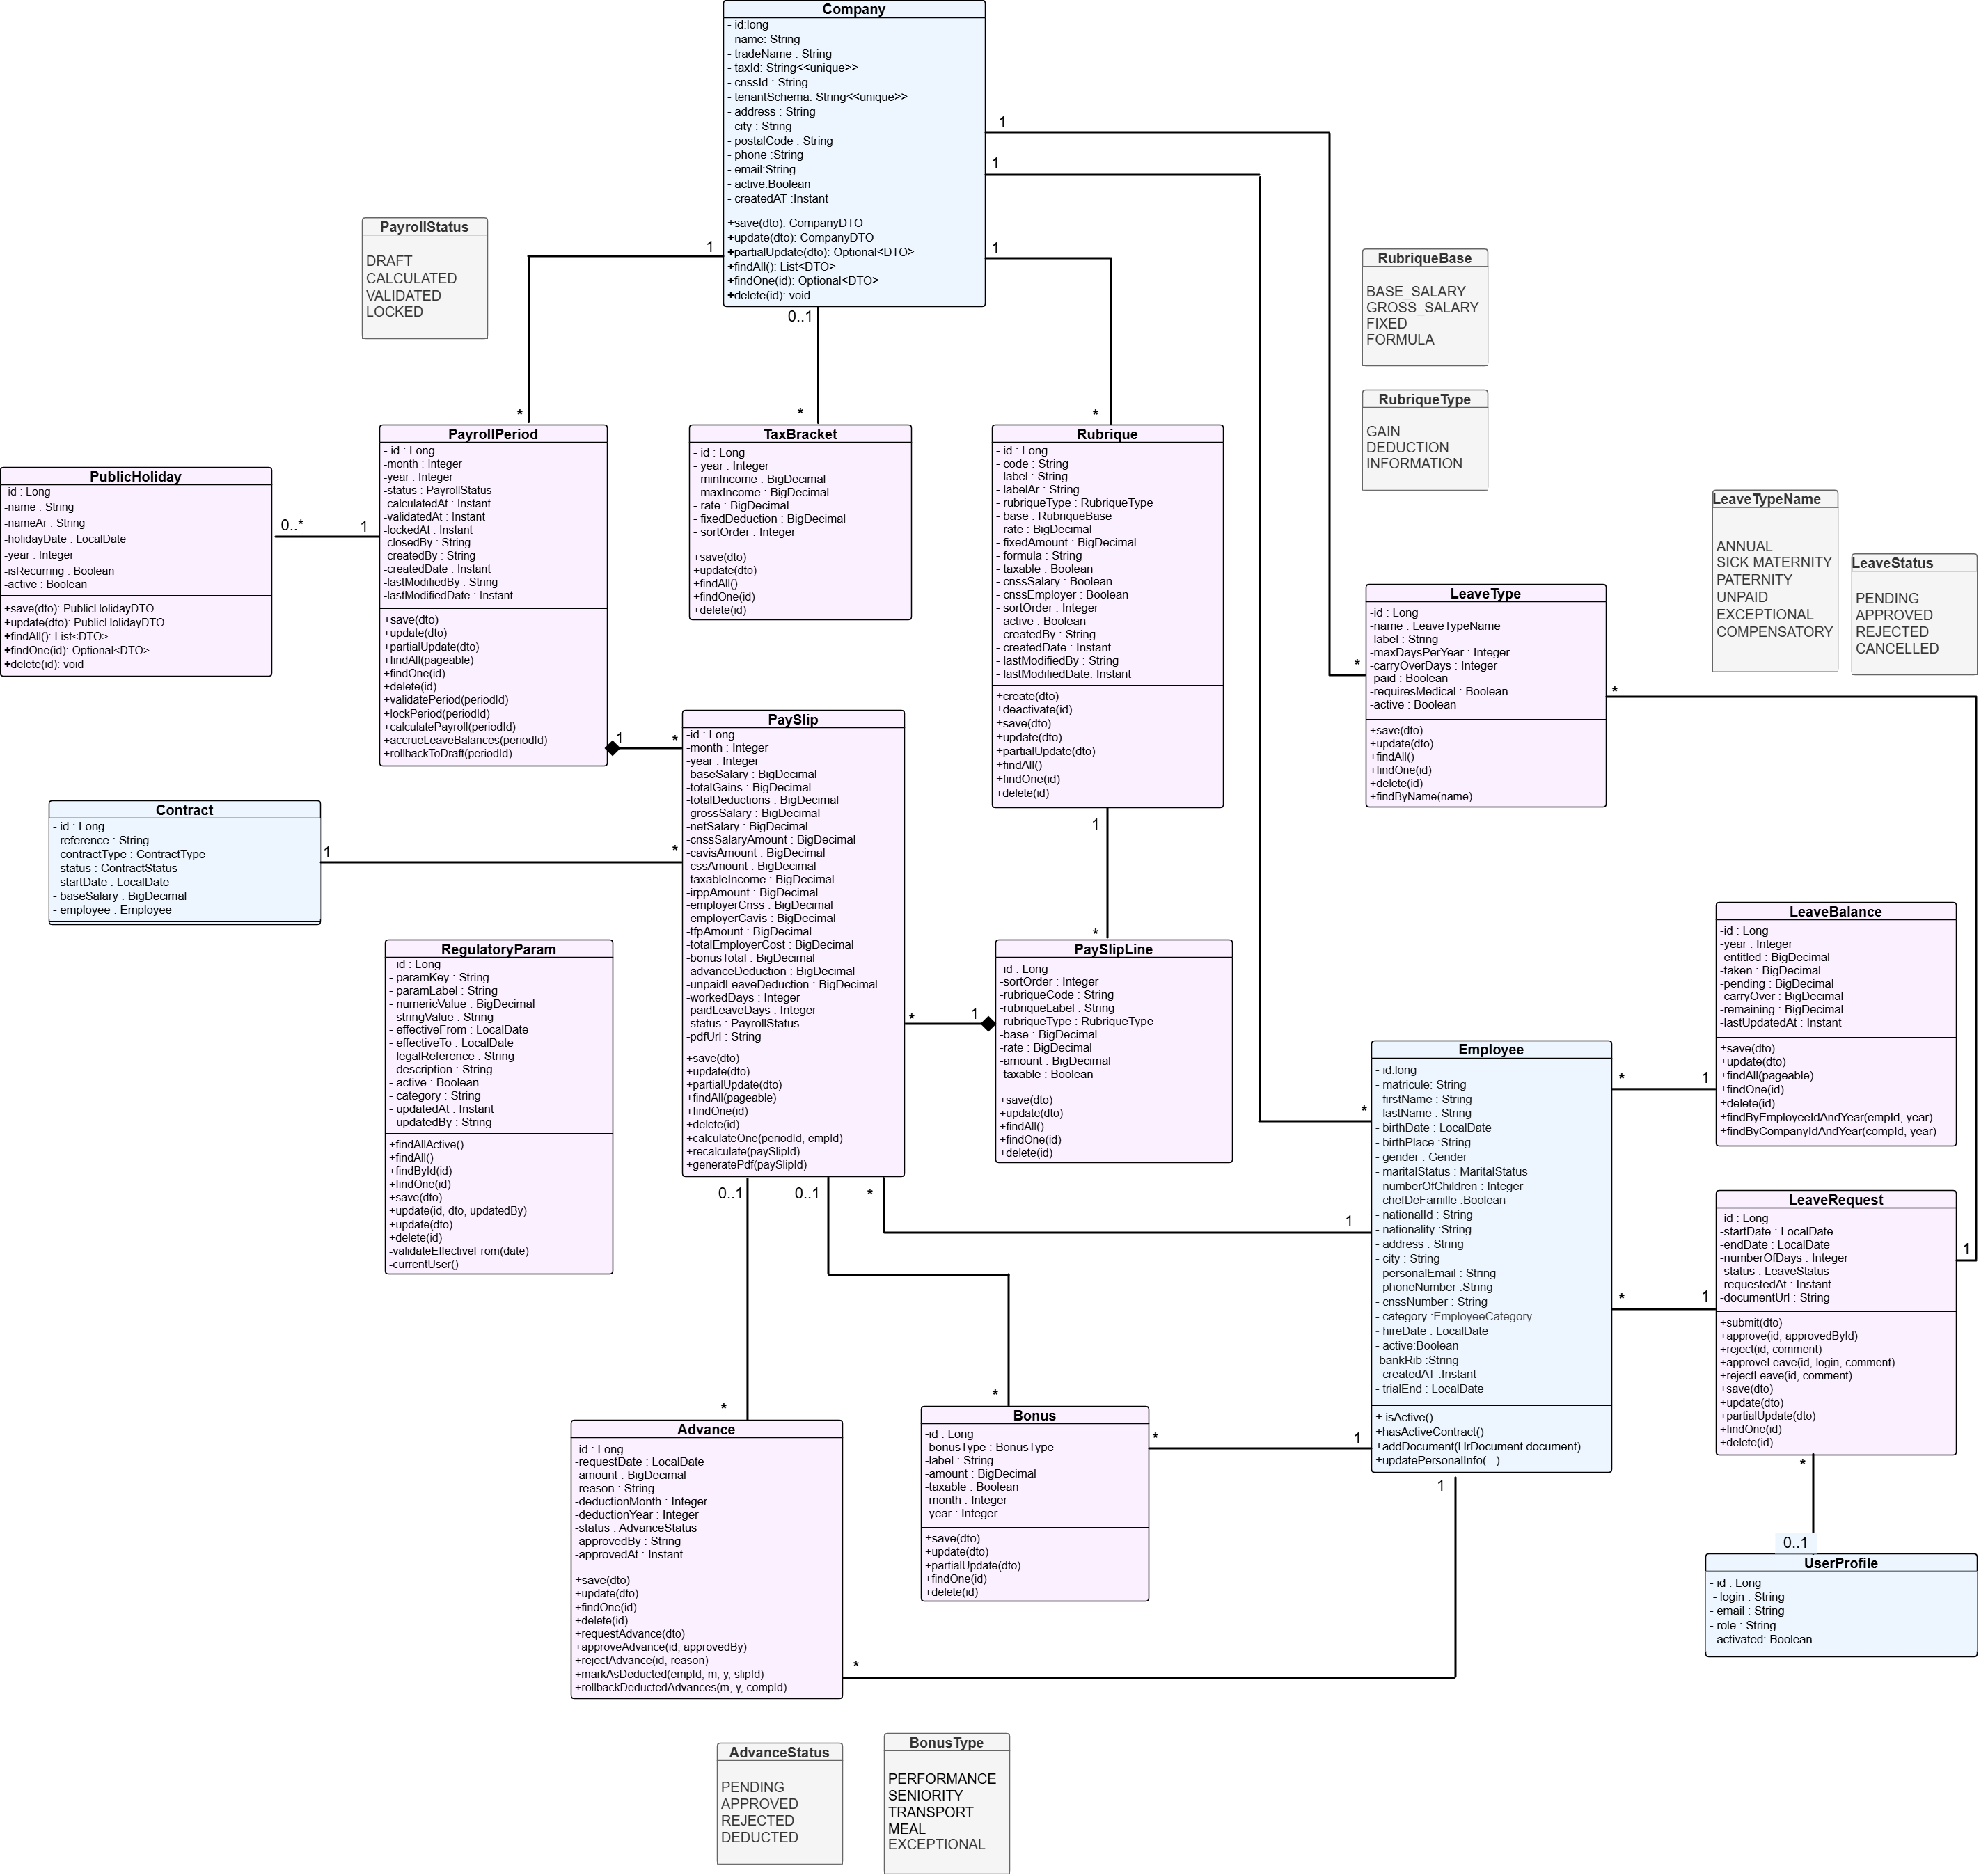
\includegraphics[width=0.99\textwidth]{classes-sprint3.png}
  \caption{Diagramme de classes du Sprint 3 --- PaieZone}
  \label{fig:classes-sprint3}
\end{figure}

Le diagramme de classes du Sprint~3 (Figure~\ref{fig:classes-sprint3})
enrichit le modèle du Sprint~2 en introduisant les entités nécessaires
au moteur de paie et à la gestion des congés.

\textbf{Entités du cycle de paie~:}
\begin{itemize}[label=\textbullet, leftmargin=0.6cm]
    \item \textbf{RegulatoryParam}~: stocke les paramètres
          réglementaires versionnés (clé, valeur numérique, date d'entrée
          en vigueur, référence légale). Plusieurs enregistrements peuvent
          coexister pour un même paramètre~; le moteur utilise toujours
          la version active à la date de la période.

    \item \textbf{TaxBracket}~: modélise les tranches progressives
          du barème IRPP (borne inférieure, borne supérieure, taux
          d'imposition, déduction fixe). Cette entité est chargée
          dynamiquement à chaque calcul de bulletin.

    \item \textbf{PayrollPeriod}~: représente une période mensuelle
          de paie (mois, année, statut~: OUVERTE /
          CALCULÉE / CLÔTURÉE, horodatage de clôture
          lockedAt). Elle est liée à la Compan
          par une association de composition.

    \item \textbf{Rubrique}~: paramètre de calcul configuré par
          la société (type~: GAIN ou RETENU, base
          de calcul, montant ou pourcentage). Elle structure les éléments
          du bulletin au-delà des cotisations légales.

    \item \textbf{Bonus}~: prime individuelle ou collective
          affectée à un employé pour une période donnée (montant, type,
          statut). Agrégée dans le brut lors du calcul.

    \item \textbf{Advance}~: demande d'avance sur salaire.
          Cycle~: PENDING~$\rightarrow$~APPROVED
          / REJECTED~$\rightarrow$~DEDUCTED lors
          du calcul du bulletin.

    \item \textbf{PaySlip}~: bulletin de paie calculé. Stocke
          tous les montants,

    \item \textbf{PaySlipLine}~: détail ligne par ligne du
          bulletin (libellé, base, taux, montant gain/retenue), permettant
          l'affichage du bulletin PDF complet.
\end{itemize}

\textbf{Entités de gestion des congés~:}
\begin{itemize}[label=\textbullet, leftmargin=0.6cm]
    \item \textbf{LeaveType}~: type de congé paramétrable
          (annuel légal, maladie, sans solde, maternité) avec quota
          annuel en jours.

    \item \textbf{LeaveBalance}~: solde de congés en temps réel
          par employé et par type de congé.

    \item \textbf{LeaveRequest}~: demande de congé soumise par
          un employé (dates, type, statut).

    \item \textbf{PublicHoliday}~: jours fériés tunisiens
          paramétrables, automatiquement exclus du décompte des jours
          de congé.
\end{itemize}

% -----------------------------------------------------------
\subsection{Diagrammes de séquences}
% -----------------------------------------------------------

Les diagrammes de séquences suivants modélisent la dynamique des
cas d'utilisation principaux du Sprint~3 selon l'architecture
N-Tiers à trois couches de PaieZone.

% -----------------------------------------------------------
\subsubsection{Diagramme de séquence : Lancer le calcul des bulletins de paie}
% -----------------------------------------------------------

La figure~\ref{fig:seq-calcul} illustre le flux de calcul automatisé
des bulletins de paie pour une période donnée.

\begin{figure}[H]
  \centering
  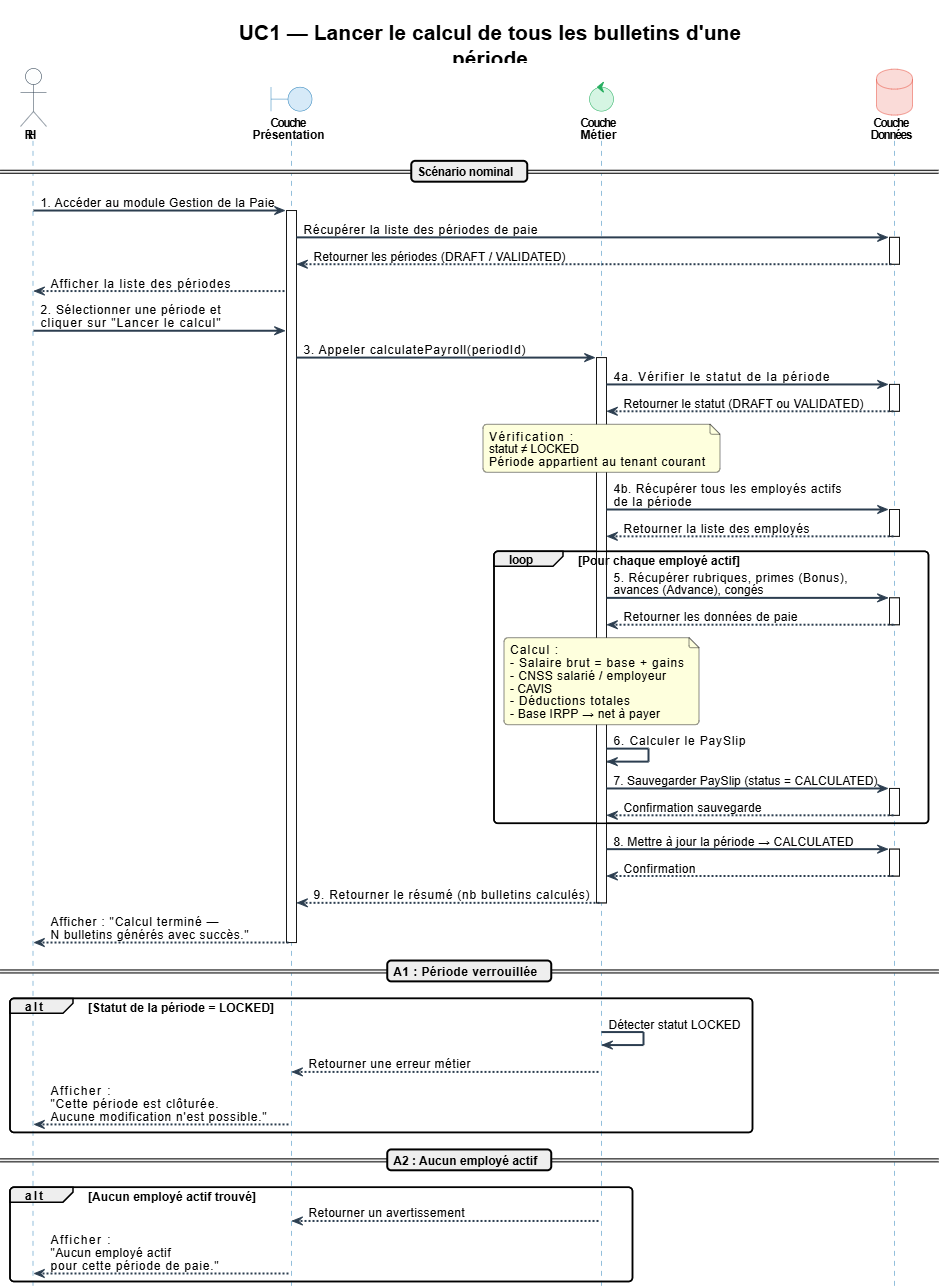
\includegraphics[width=0.78\textwidth]{seq-sp3-uc1.png}
  \caption{Diagramme de séquence --- Lancer le calcul des bulletins de paie}
  \label{fig:seq-calcul}
\end{figure}

Ce diagramme illustre l'ordonnancement du traitement de la paie,
pilier central du Sprint~3. Le moteur de calcul automatise la
transformation des données contractuelles en bulletins de paie nets,
en appliquant rigoureusement les barèmes réglementaires à l'ensemble
des employés actifs. Ce flux garantit l'intégrité des résultats
financiers ainsi que la mise à jour cohérente des statuts de la
période de paie.

% -----------------------------------------------------------
\subsubsection{Diagramme de séquence : Clôturer une période de paie}
% -----------------------------------------------------------

La figure~\ref{fig:seq-cloture} illustre le flux de clôture d'une
période de paie.

\begin{figure}[H]
  \centering
  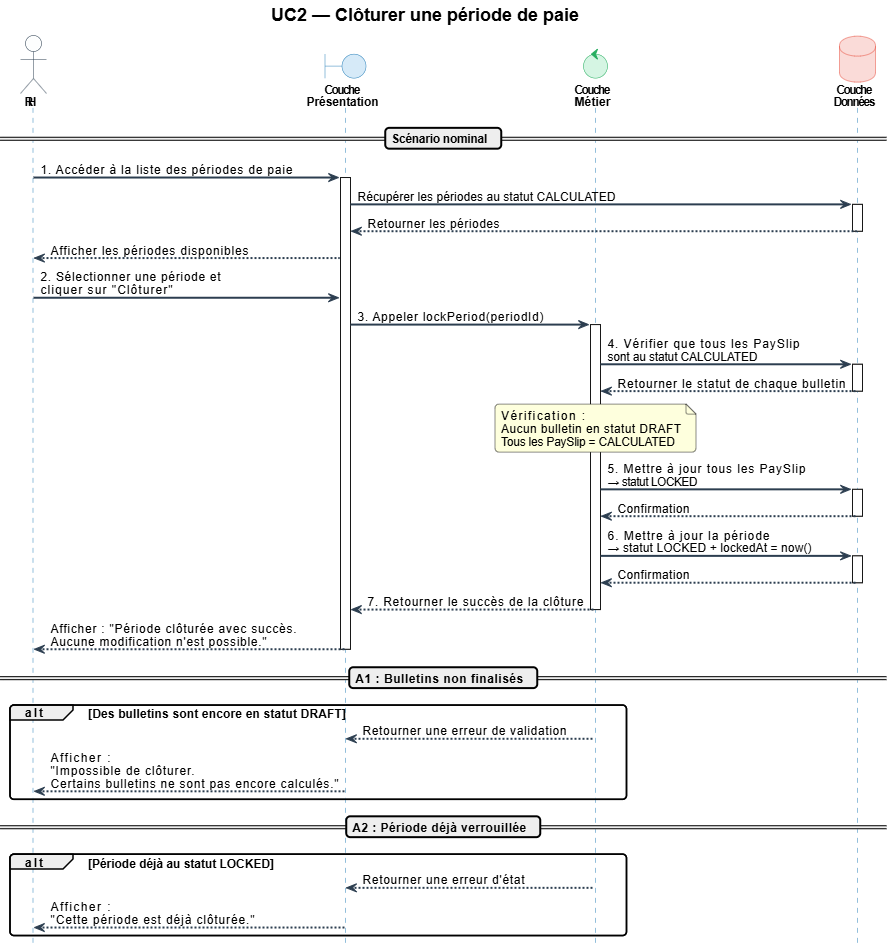
\includegraphics[width=0.90\textwidth]{seq-sp3-uc2.png}
  \caption{Diagramme de séquence --- Clôturer une période de paie }
  \label{fig:seq-cloture}
\end{figure}

Ce diagramme détaille le processus de clôture définitive d'une période
de paie, garantissant l'intégrité et l'immuabilité des résultats
financiers. Le flux assure la validation préalable de l'état des
bulletins avant d'opérer un verrouillage global, interdisant ainsi
toute modification ultérieure des données de paie.

% -----------------------------------------------------------
\subsubsection{Diagramme de séquence : Demande et traitement d’une avance sur salaire}
% -----------------------------------------------------------

La figure~\ref{fig:seq-avance2} illustre le flux de demande et de
traitement d'une avance sur salaire.

\begin{figure}[H]
  \centering
  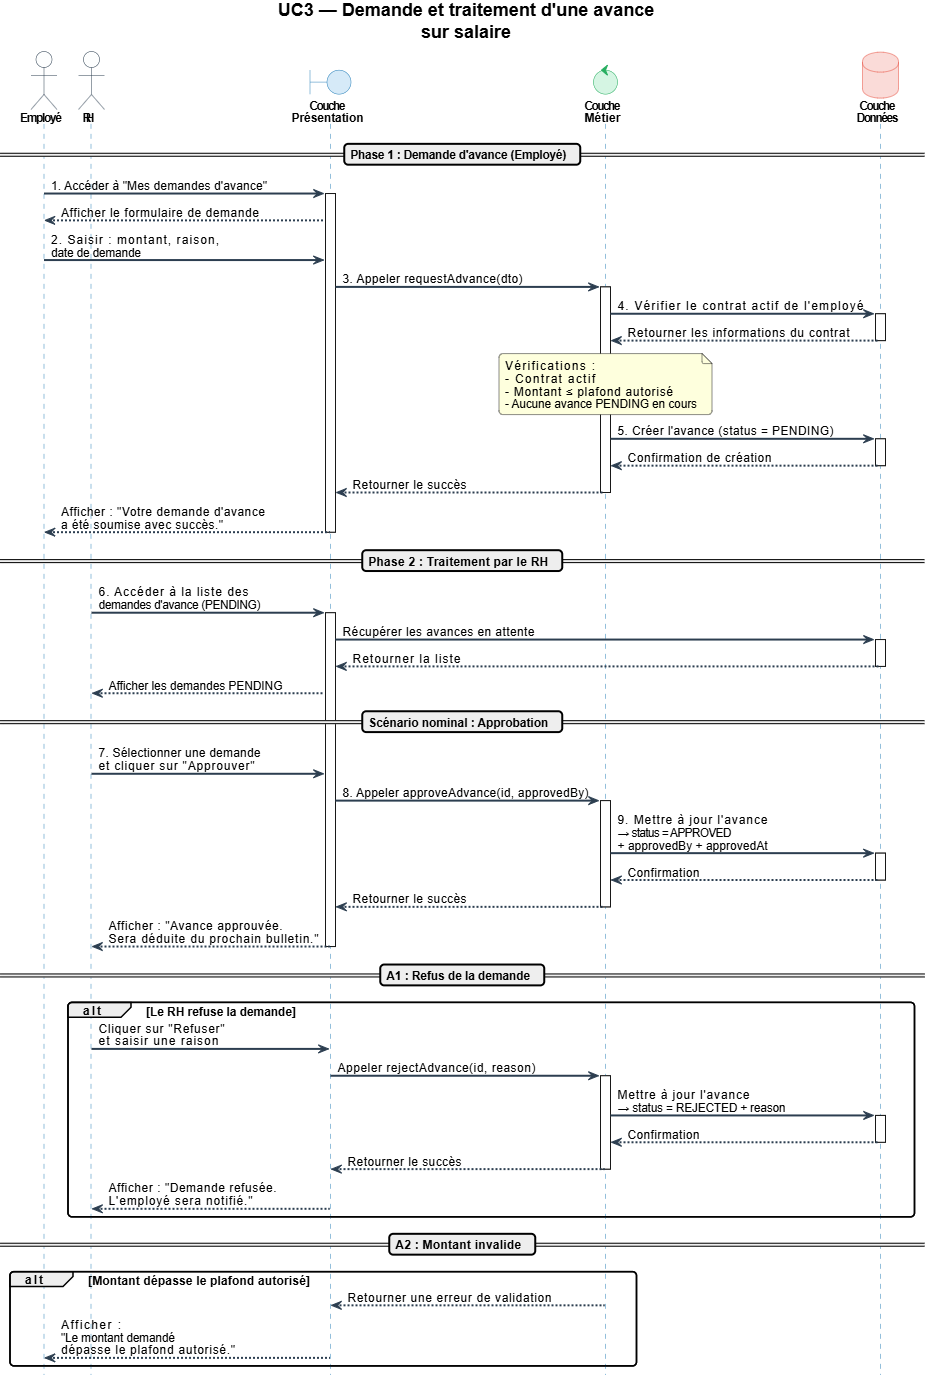
\includegraphics[width=0.775\textwidth]{seq-sp3-uc3.png}
  \caption{Diagramme de séquence --- Demande et traitement d'une avance sur salaire}
  \label{fig:seq-avance2}
\end{figure}

Ce diagramme illustre le processus de gestion des avances sur salaire.
Le flux débute par la soumission de la demande par l'\textbf{Employé},
soumise à des contrôles d'éligibilité automatiques (contrat actif,
plafond autorisé), et se conclut par la décision du \textbf{RH}
(approbation ou refus). L'approbation déclenche l'intégration automatique
de l'avance dans le prochain cycle de paie avec passage au statut DEDUCTE lors du calcul du bulletin.

% ============================================================
\section{Étude et réalisation}
\label{sec:s3-realisation}
% ============================================================

Cette section détaille les réalisations concrètes du troisième sprint,
marquant l'aboutissement du c\oe{}ur métier de la plateforme. Les travaux
ont porté sur~: l'implémentation du moteur de calcul de paie conforme
à la Loi de Finances 2026, le traitement en lot transactionnel des
bulletins, la génération PDF
des bulletins, la configuration des paramètres
réglementaires versionnés, et l'automatisation des processus de
gestion des congés avec mise à jour dynamique des soldes.

% -----------------------------------------------------------
\subsection{Gestion des paramètres réglementaires}
% -----------------------------------------------------------

\begin{figure}[H]
  \centering
  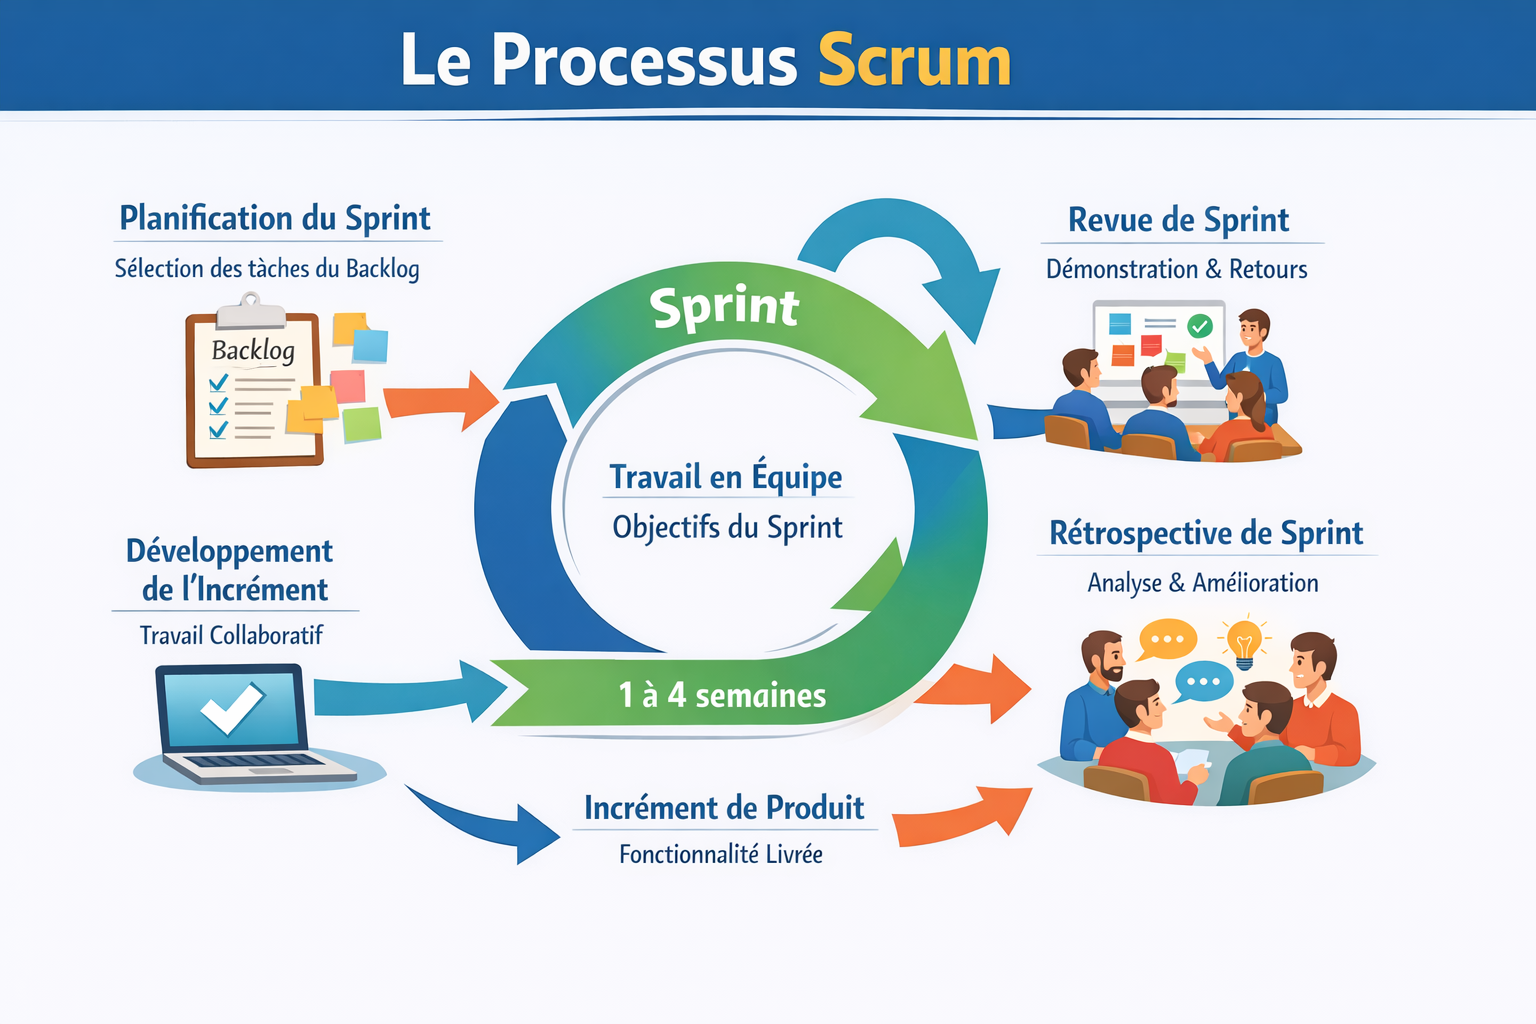
\includegraphics[width=0.70\textwidth]{scrum.png}
  \caption{Interface de gestion des paramètres réglementaires}
  \label{fig:ui-params}
\end{figure}

La figure~\ref{fig:ui-params} présente l'interface de gestion des
paramètres réglementaires, accessible exclusivement au Super Admin.
Elle permet de consulter, ajouter et modifier les constantes légales
(taux CNSS, CAVIS, CSS, TFP, barème IRPP, SMIG) sans redéploiement.
Chaque modification est horodatée et tracée dans le journal d'audit.

% -----------------------------------------------------------
\subsection{Gestion des périodes de paie}
% -----------------------------------------------------------

\begin{figure}[H]
  \centering
  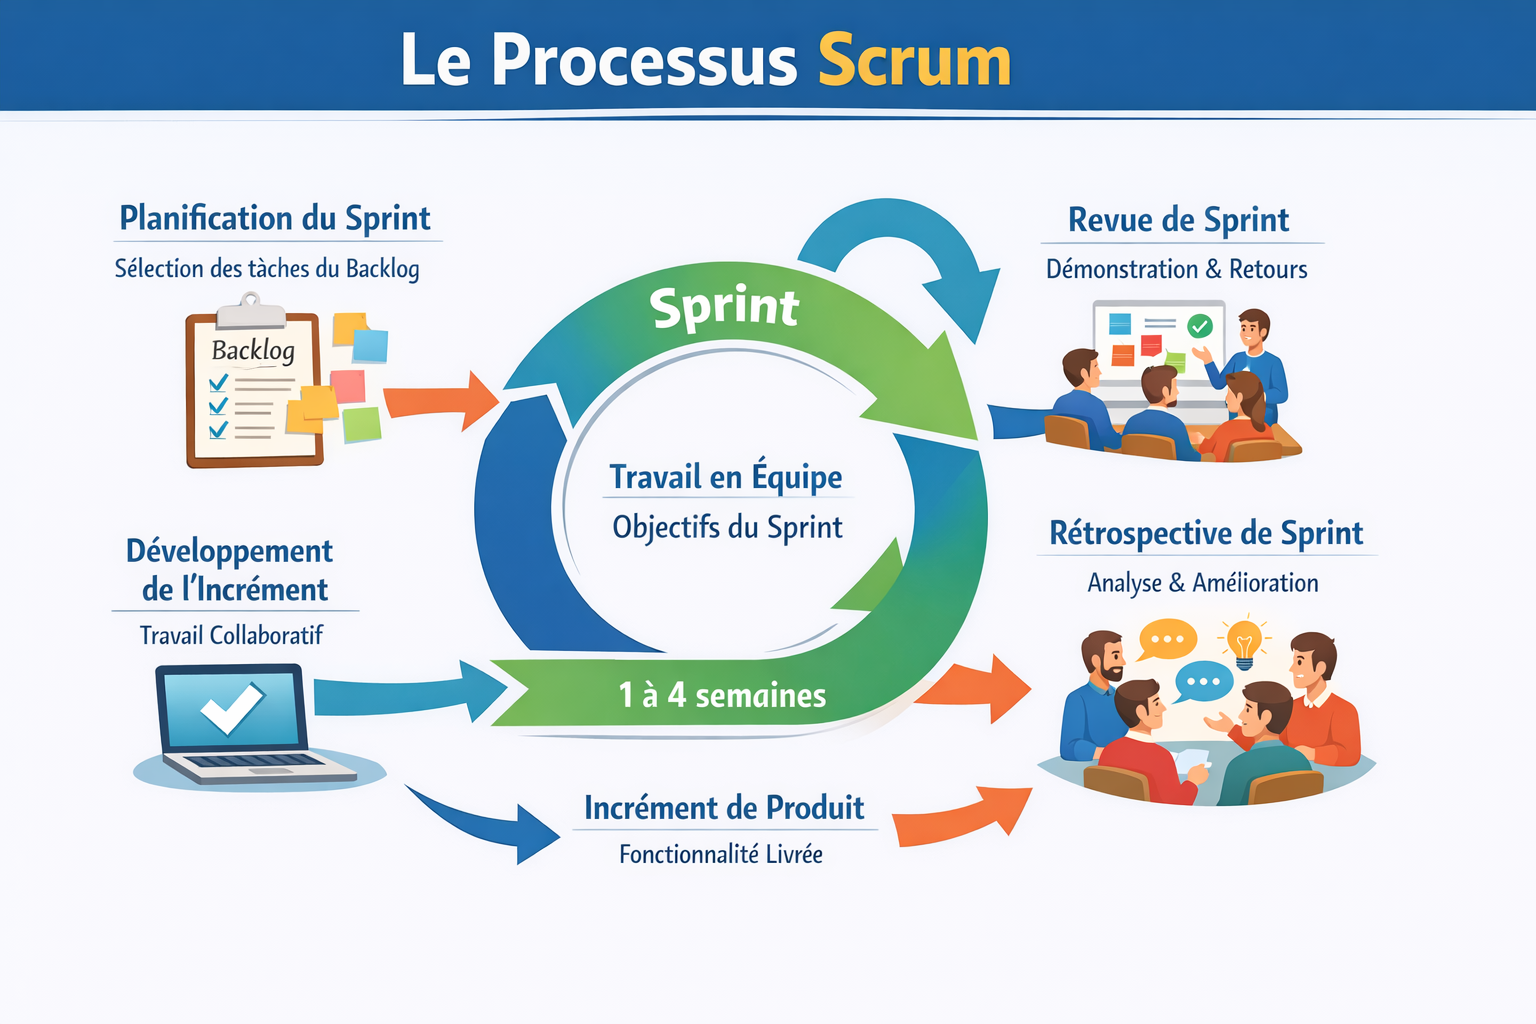
\includegraphics[width=0.70\textwidth]{scrum.png}
  \caption{Interface de gestion des périodes de paie}
  \label{fig:ui-periodes}
\end{figure}

La figure~\ref{fig:ui-periodes} présente le module de gestion des
périodes de paie. Le RH peut créer une nouvelle période mensuelle,
suivre son évolution selon trois statuts successifs~:
OUVERTE (calcul possible), CALCULÉE (bulletins
générés, clôture autorisée) et CLÔTURÉE (verrouillage
définitif). Ce mécanisme garantit
l'immuabilité des données de paie validées.

% -----------------------------------------------------------
\subsection{Calcul et visualisation des bulletins de paie}
% -----------------------------------------------------------

\begin{figure}[H]
  \centering
  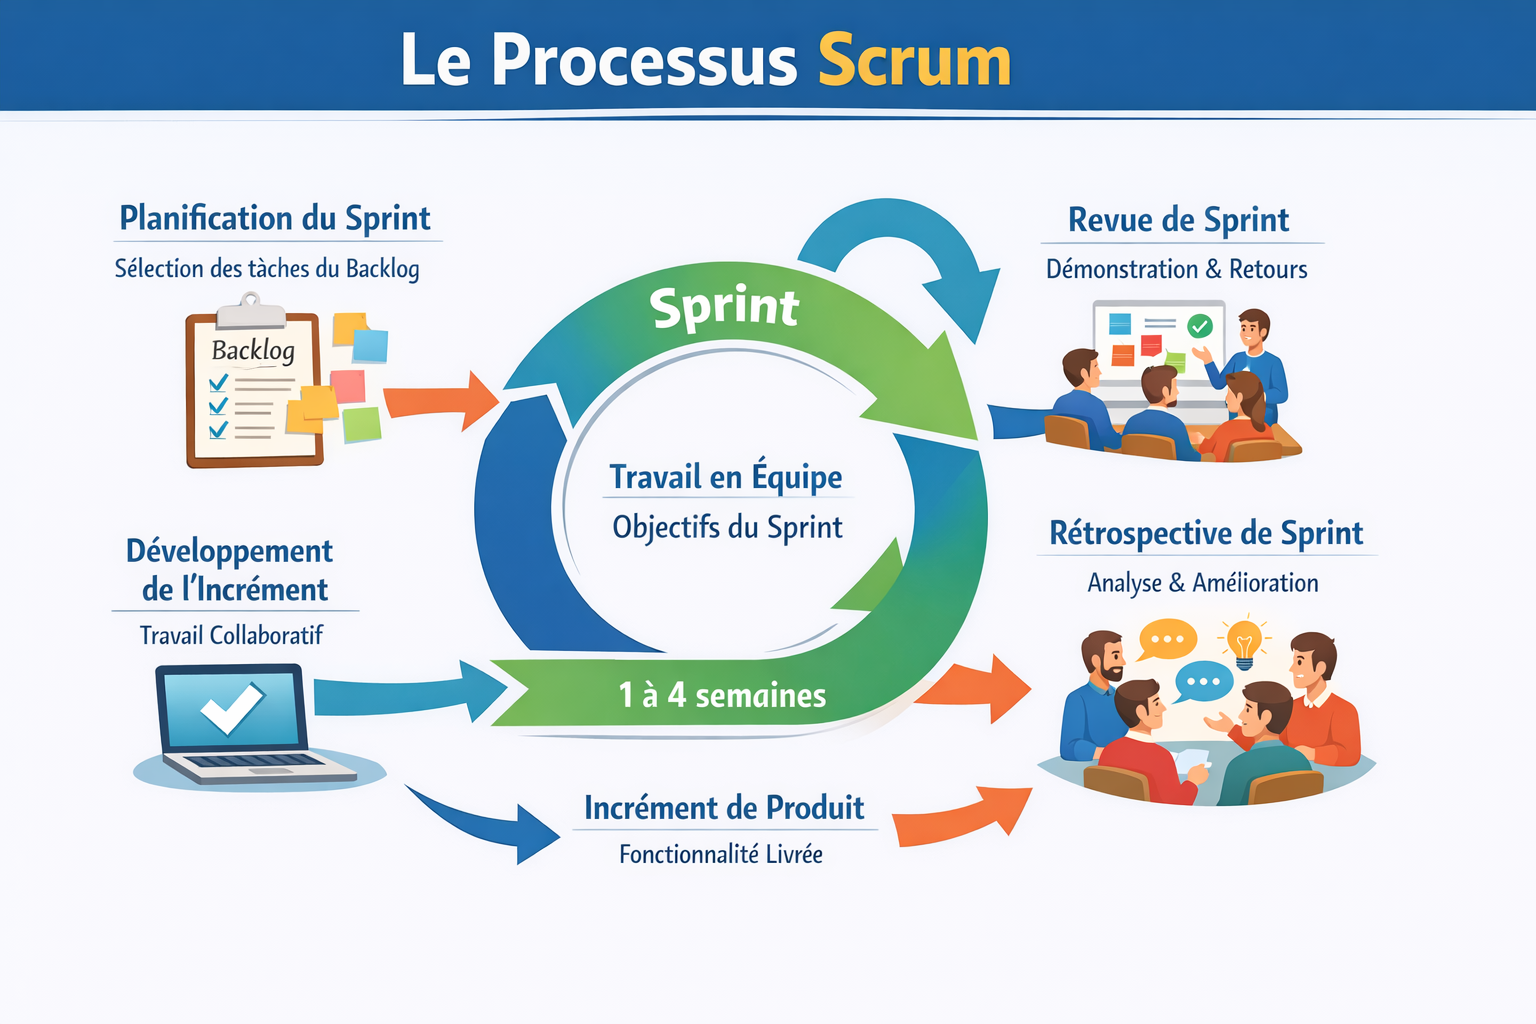
\includegraphics[width=0.70\textwidth]{scrum.png}
  \caption{Interface de calcul et de visualisation des bulletins de paie}
  \label{fig:ui-bulletins}
\end{figure}

La figure~\ref{fig:ui-bulletins} présente l'interface de calcul des
bulletins de paie. Le RH lance le calcul en lot, visualise les bulletins
générés avec le détail des cotisations et du montant net, et peut
exporter chaque bulletin en PDF ou déclencher l'envoi groupé.

% -----------------------------------------------------------
\subsection{Gestion des primes et des avances}
% -----------------------------------------------------------

\begin{figure}[H]
  \centering
  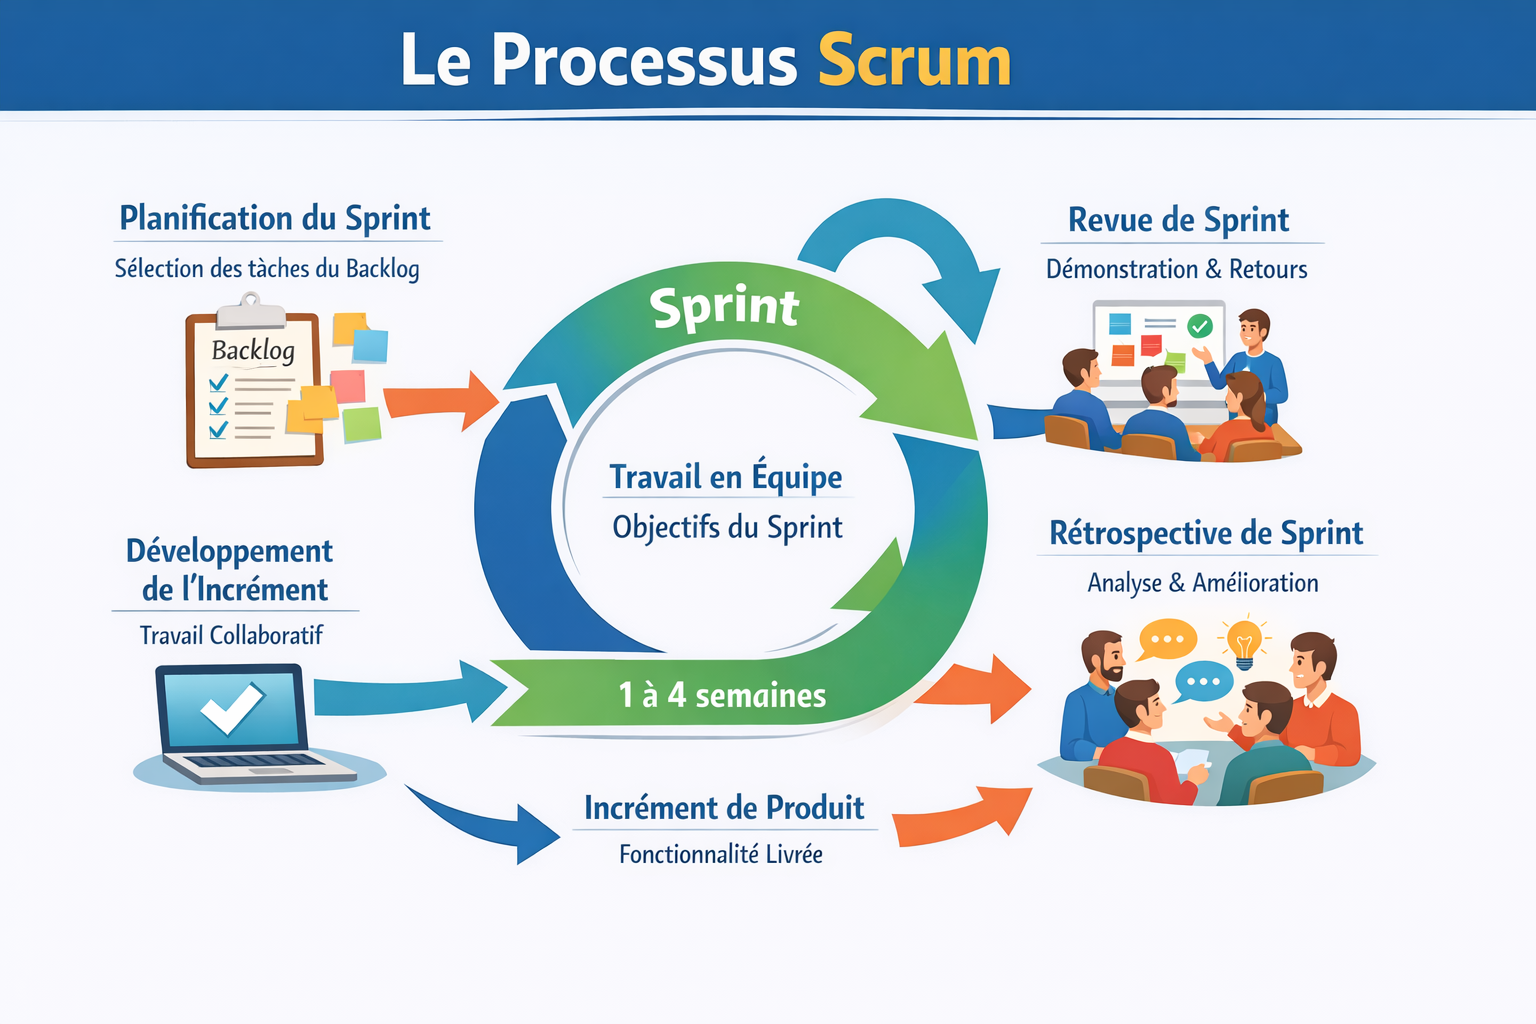
\includegraphics[width=0.70\textwidth]{scrum.png}
  \caption{Interface de gestion des primes et des avances}
  \label{fig:ui-primes}
\end{figure}

La figure~\ref{fig:ui-primes} présente le module de gestion des
éléments variables de la paie. Le RH peut ajouter des primes
individuelles ou collectives et traiter les demandes d'avance soumises
par les employés (validation ou refus). Les montants validés sont
automatiquement intégrés dans le calcul du bulletin de la période
courante.

% -----------------------------------------------------------
\subsection{Gestion des congés et des absences}
% -----------------------------------------------------------

\begin{figure}[H]
  \centering
  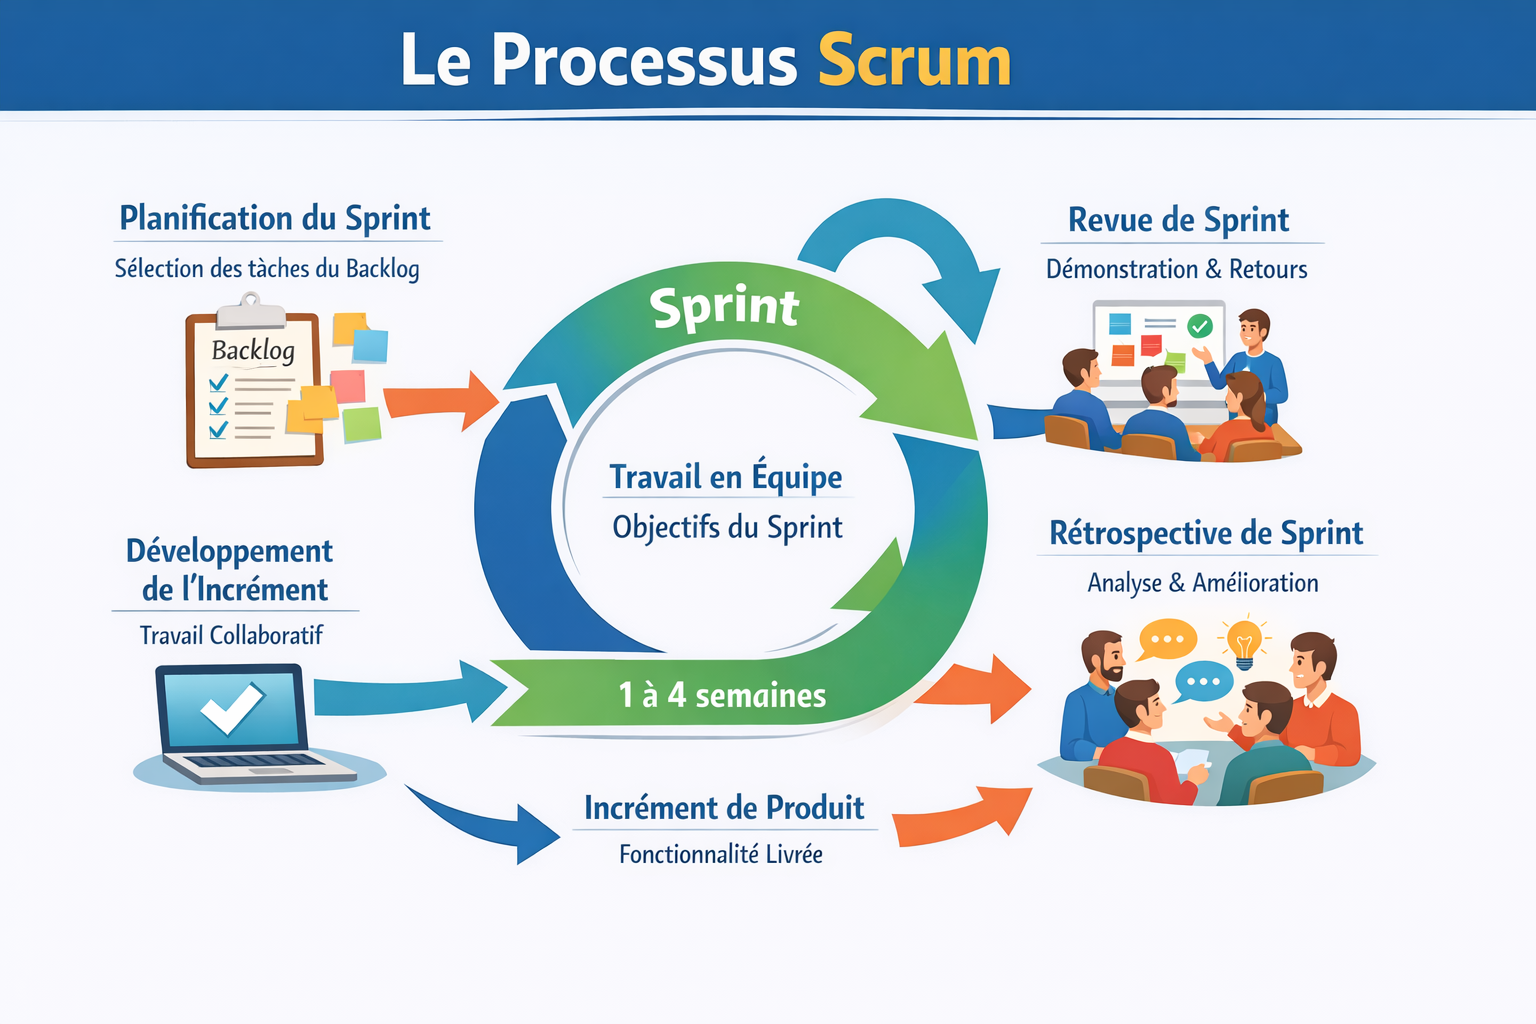
\includegraphics[width=0.70\textwidth]{scrum.png}
  \caption{Interface de gestion des congés et des absences}
  \label{fig:ui-conges}
\end{figure}

La figure~\ref{fig:ui-conges} présente le module de gestion des congés.
L'Employé dispose d'un calendrier interactif pour soumettre ses demandes
et consulter son solde en temps réel. Le RH accède à un tableau de bord
des demandes en attente, avec les actions de validation et de refus.
Les jours fériés configurés sont automatiquement exclus du décompte
des jours de congé.

% ============================================================
\section{Tests et Validation}
\label{sec:s3-tests}
% ============================================================

La phase de tests du Sprint~3 accorde une importance particulière
à la fiabilité du moteur de calcul de paie, dont les résultats ont
des implications financières et légales directes pour les sociétés
clientes de PaieZone.

% -----------------------------------------------------------
\subsection{Plan de tests}
% -----------------------------------------------------------

Trois types de tests ont été mis en \oe{}uvre~: les \textbf{tests
unitaires} du moteur de calcul, les \textbf{tests
d'intégration} des flux métier complets, et les \textbf{tests
fonctionnels} des interfaces Angular.

Le tableau~\ref{tab:tests-sprint3} présente le plan de tests du Sprint~3.

\begin{small}
\renewcommand{\arraystretch}{1.3}
\begin{longtable}{|>{\bfseries}p{1.5cm}|p{1.2cm}|p{2cm}|p{4.5cm}|p{2.5cm}|p{1.5cm}|}

\hline
\rowcolor[gray]{0.9}\textbf{ID} & \textbf{US} & \textbf{Type} &
\textbf{Description} & \textbf{Résultat attendu} & \textbf{Statut} \\ \hline
\endfirsthead
\hline
\rowcolor[gray]{0.9}\textbf{ID} & \textbf{US} & \textbf{Type} &
\textbf{Description} & \textbf{Résultat attendu} & \textbf{Statut} \\ \hline
\endhead
\hline
\endfoot
\hline
\caption{Plan de tests du Sprint 3 }
\label{tab:tests-sprint3} 
\endlastfoot
TC-01 & 10.2 & Unitaire & Ajout d'un paramètre avec un taux valide & Paramètre enregistré, audit tracé & OK \\ \hline
TC-02 & 10.3 & Unitaire & Modification avec taux hors bornes & Erreur de validation bloquante & OK \\ \hline
TC-03 & 11.1 & Intégration & Création d'une période de paie & Période créée au statut \texttt{OUVERTE} & OK \\ \hline
TC-04 & 11.3 & Intégration & Clôture d'une période & Statut \texttt{CLÔTURÉE}, modifications rejetées & OK \\ \hline
TC-05 & 11.4 & Unitaire & Calcul du salaire net avec prime et avance & Net = Brut + Prime - CNSS - CAVIS - CSS - IRPP - Avance & OK \\ \hline
TC-06 & 11.4 & Intégration & Calcul par lot pour 10 employés & 10 bulletins générés sans erreur & OK \\ \hline
TC-07 & 11.4 & Intégration & Calcul sans paramètres configurés & Erreur bloquante + message explicite & OK \\ \hline
TC-08 & 11.12 & Fonctionnel & Génération du bulletin PDF & PDF conforme au template réglementaire & OK \\ \hline
TC-09 & 11.13 & Fonctionnel & Génération du fichier CNSS & Fichier au format réglementaire & OK \\ \hline
TC-10 & 12.2 & Intégration & Demande de congé avec solde insuffisant & Demande bloquée & OK \\ \hline
TC-11 & 12.3 & Intégration & Validation d'un congé & Solde décrémenté + notification envoyée & OK \\ \hline
TC-12 & 12.5 & Intégration & Congé couvrant un jour férié & Jour férié exclu du décompte & OK \\ \hline
\end{longtable}
\end{small}
\renewcommand{\arraystretch}{1.0}

La stratégie de validation du Sprint~3 s'est concentrée sur la fiabilité
du moteur de calcul et la conformité légale des documents produits. Une
attention particulière a été portée aux scénarios critiques, tels que
la gestion simultanée des éléments variables de paie, l'intégrité des
calculs en l'absence de paramètres configurés, et l'irréversibilité du
processus de clôture.

% -----------------------------------------------------------
\subsection{Tests automatisés}
% -----------------------------------------------------------

Le Sprint~3 concentre les calculs financiers les plus critiques de \pz{}
(CNSS, IRPP, CSS, génération PDF). Deux classes de tests automatisés ont
été développées avec JUnit~5 et Mockito.

\paragraph{TunisianTaxServiceTest --- 8 cas de test}
Ces tests vérifient la conformité des calculs fiscaux à la
\textbf{Loi de Finances 2026} (JORT n°3-2026). Chaque taux est testé
indépendamment pour éviter toute régression lors des mises à jour réglementaires
annuelles~:

\renewcommand{\arraystretch}{1.2}
\begin{small}
\begin{xltabular}{\textwidth}{|c|X|p{4cm}|c|}
\hline
\rowcolor[gray]{0.9}
\textbf{ID} & \textbf{Scénario} & \textbf{Résultat attendu} & \textbf{Statut} \\ \hline
\endfirsthead \hline
\rowcolor[gray]{0.9}
\textbf{ID} & \textbf{Scénario} & \textbf{Résultat attendu} & \textbf{Statut} \\ \hline
\endhead \hline \endfoot \hline
\caption{Tests automatisés --- TunisianTaxServiceTest}\label{tab:auto-tax}\endlastfoot
TA-S3-01 & CNSS salarial, salaire 1~500~TND (sous plafond)
    & 145,200 TND (9,68\,\%) & \textcolor{green!60!black}{\textbf{OK}} \\ \hline
TA-S3-02 & CNSS salarial, salaire 7~000~TND (au-dessus plafond 5~000 TND)
    & 484,000 TND (plafonné) & \textcolor{green!60!black}{\textbf{OK}} \\ \hline
TA-S3-03 & CSS à 0,5\,\% sur revenu imposable 1~806,400 TND
    & 9,032 TND & \textcolor{green!60!black}{\textbf{OK}} \\ \hline
TA-S3-04 & IRPP annuel $<$ 5~000 TND (tranche exonérée)
    & 0 TND & \textcolor{green!60!black}{\textbf{OK}} \\ \hline
TA-S3-05 & IRPP dans la tranche à 15\,\%
    & Montant conforme au barème LF 2026 & \textcolor{green!60!black}{\textbf{OK}} \\ \hline
TA-S3-06 & Chef de famille avec 2 enfants paie moins qu'un célibataire
    & IRPP chef $<$ IRPP célibataire & \textcolor{green!60!black}{\textbf{OK}} \\ \hline
TA-S3-07 & Calcul intégré : 2~000 TND, marié, 2~enfants
    & Net = 1~543,685 TND & \textcolor{green!60!black}{\textbf{OK}} \\ \hline
TA-S3-08 & IRPP mensuel dans la tranche à 25\,\%
    & Montant conforme au barème & \textcolor{green!60!black}{\textbf{OK}} \\ \hline
\end{xltabular}
\end{small}
\renewcommand{\arraystretch}{1.0}

\paragraph{PdfExportServiceTest --- 8 cas de test}
Ces tests vérifient que chaque PDF généré est un fichier valide
(signature binaire \texttt{\%PDF}) et que les cas d'erreur sont
correctement gérés (bulletin introuvable $\rightarrow$
\texttt{EntityNotFoundException}).

\renewcommand{\arraystretch}{1.2}
\begin{small}
\begin{xltabular}{\textwidth}{|c|X|p{4cm}|c|}
\hline
\rowcolor[gray]{0.9}
\textbf{ID} & \textbf{Scénario} & \textbf{Résultat attendu} & \textbf{Statut} \\ \hline
\endfirsthead \hline
\rowcolor[gray]{0.9}
\textbf{ID} & \textbf{Scénario} & \textbf{Résultat attendu} & \textbf{Statut} \\ \hline
\endhead \hline \endfoot \hline
\caption{Tests automatisés --- PdfExportServiceTest}\label{tab:auto-pdf}\endlastfoot
TA-S3-09 & Génération bulletin pour un employé valide
    & PDF non vide, commence par \texttt{\%PDF} & \textcolor{green!60!black}{\textbf{OK}} \\ \hline
TA-S3-10 & Génération bulletin, ID inexistant
    & \texttt{EntityNotFoundException} levée & \textcolor{green!60!black}{\textbf{OK}} \\ \hline
TA-S3-11 & Génération bulletin avec heures supplémentaires
    & PDF valide incluant la ligne HS & \textcolor{green!60!black}{\textbf{OK}} \\ \hline
TA-S3-12 & Génération attestation de travail
    & PDF valide & \textcolor{green!60!black}{\textbf{OK}} \\ \hline
TA-S3-13 & Génération attestation, employé inconnu
    & \texttt{EntityNotFoundException} levée & \textcolor{green!60!black}{\textbf{OK}} \\ \hline
TA-S3-14 & Journal de paie pour 1 bulletin
    & PDF valide & \textcolor{green!60!black}{\textbf{OK}} \\ \hline
TA-S3-15 & Journal de paie sans aucun bulletin
    & \texttt{IllegalStateException} levée & \textcolor{green!60!black}{\textbf{OK}} \\ \hline
TA-S3-16 & Génération en masse (bulk) pour 2 bulletins
    & PDF fusionné valide & \textcolor{green!60!black}{\textbf{OK}} \\ \hline
\end{xltabular}
\end{small}
\renewcommand{\arraystretch}{1.0}

\textbf{Résultat global Sprint~3~:} 16/16 tests automatisés passés
(\textcolor{green!60!black}{\textbf{OK}}), couverture estimée à
\textbf{85\,\%} pour \texttt{TunisianTaxService} et \textbf{65\,\%}
pour \texttt{PdfExportService}.

% ============================================================
\section{Rituels Agiles et Clôture du Sprint}
\label{sec:s3-rituels}
% ============================================================

En parfaite adéquation avec le cadre méthodologique Scrum, le Sprint 3 s'est conclu par l'exécution des rituels de clôture standards. Ces rituels incluent la revue de sprint, dédiée à la validation des livrables en présence des parties prenantes, et la rétrospective, axée sur l'analyse critique et l'amélioration continue des processus de l'équipe de développement.

% -----------------------------------------------------------
\subsection{Revue du Sprint (Sprint Review)}
% -----------------------------------------------------------

La Sprint Review a permis de valider les livrables du Sprint~3 devant
le Product Owner~: moteur de calcul de paie, génération des bulletins
PDF et du fichier CNSS, ainsi que le module de gestion des congés.
L'ensemble des vingt-deux User Stories a été accepté.

% -----------------------------------------------------------
\subsection{Rétrospective du Sprint (Sprint Retrospective)}

L'équipe a mené une réflexion collective sur le déroulement du Sprint~3~:

\begin{itemize}[label=\textbullet, leftmargin=0.6cm]

    \item \textbf{Ce qui a bien fonctionné~:}
    \begin{itemize}[label=\textbullet, leftmargin=0.8cm]
        \item Le calcul en lot transactionnel a démontré sa fiabilité pour
              le traitement simultané de l'ensemble des bulletins de paie.
        \item La communication fluide avec le Product Owner a facilité la
              validation rapide des livrables.
    \end{itemize}

    \item \textbf{Problèmes rencontrés~:}
    \begin{itemize}[label=\textbullet, leftmargin=0.8cm]
        \item La complexité du calcul IRPP par tranches progressives a été
              sous-estimée lors du Sprint Planning.
        \item La validation du format du fichier CNSS a nécessité plusieurs
              cycles de correction en fin de sprint.
    \end{itemize}

    \item \textbf{Actions d'amélioration pour le Sprint~4~:}
    \begin{itemize}[label=\textbullet, leftmargin=0.8cm]
        \item Lors des tests, la nécessité d'intégrer les conventions
              sectorielles (jours ouvrables, primes spécifiques) a été
              identifiée~; cette fonctionnalité sera implémentée dans
              le Sprint~4.
    \end{itemize}

\end{itemize}
% ============================================================
\section*{Conclusion}
\label{sec:s3-conclusion}
\addcontentsline{toc}{section}{Conclusion}
% ============================================================
Ce cinquième chapitre a présenté les travaux du Sprint~3, dédié au
c\oe{}ur métier de PaieZone~RH~: paramétrage réglementaire, calcul
automatisé de la paie et gestion des congés. Les vingt-deux User
Stories ont été validées par le Product Owner. Le chapitre suivant
présente le Sprint~4, qui finalise la plateforme avec la comptabilité
intégrée, les déclarations réglementaires, l'intégration des conventions
sectorielles et le déploiement de l'assistant conversationnel PaieBot.